\documentclass[aspectratio=169]{beamer}

\usepackage[utf8]{inputenc}

\usepackage{amsfonts}
\usepackage{amsmath}
\usepackage{amssymb}
\usepackage{color}
\usepackage{listings}
\usepackage{tikz}
\usepackage{hyperref}

\usetikzlibrary {arrows,arrows.meta,positioning,shapes.misc}

\newif\ifnotes
  \notesfalse
%  \notestrue

\ifnotes
\usepackage{pgfpages}
\setbeameroption{show notes}
\setbeameroption{show notes on second screen=right}
\fi

\usetheme{Rochester}
\usecolortheme{beaver}

\addtobeamertemplate{navigation symbols}{}{%
    \usebeamerfont{footline}%
    \usebeamercolor[fg]{footline}%
    \hspace{1em}%
    \insertframenumber/\inserttotalframenumber
}

\lstloadlanguages{C++}
    \lstset{%
        language={C++},
        basicstyle=\ttfamily,
        keywordstyle=\color{blue},
        showstringspaces=false,
        escapechar={§},
        escapeinside={(*@}{@*)}
    }

\newif\iftransitions
 \transitionstrue
% \transitionsfalse

\newcommand{\cpause}{\iftransitions \pause \fi}

\newcommand{\cuncover}[2]{\iftransitions \uncover<#1>{#2} \else #2 \fi}

\newif\iffast
% \fasttrue

\title{Barest Metal Deployment -}
\subtitle{Building A CPU From Scratch}
\author{Andreas Weis}
\institute{ekxide IO GmbH}
\date{MUC++ October 2026}
\titlegraphic{
\includegraphics[height=.15\textheight]{../resources/mucpp-logo-128x128.png}}

\iffalse
Outline:


\fi

\begin{document}

\frame{\titlepage}

\iftrue %crop
\fi

% \iffalse % !!!!!!!!!!!!!!

\begin{frame}[fragile]
  \frametitle{About me - Andreas Weis (he/him)}

  \begin{itemize}
    \setlength\itemsep{1.5em}

    \item \href{https://stackoverflow.com/users/577603/comicsansms}{
\includegraphics[height=.05\textheight]{../resources/so-icon.png}} \href{https://github.com/ComicSansMS}{
\includegraphics[height=.05\textheight]{../resources/github-icon.png}} \href{https://bsky.app/profile/comicsansms.bsky.social}{
\includegraphics[height=.05\textheight]{../resources/Bluesky_Logo.png}} ComicSansMS

    \item \href{mailto:cpp@andreas-weis.net}{\raisebox{-0.25em}{
\includegraphics[height=.06\textheight]{../resources/email-icon.png}} cpp@andreas-weis.net}

    \item \href{https://www.meetup.com/MUCplusplus/}{
\includegraphics[height=.05\textheight]{../resources/meetup-icon.png}} Co-organizer of the \href{https://www.meetup.com/MUCplusplus/}{Munich C++ User Group}

    \item Work for \href{https://ekxide.io/}{\raisebox{-0.35em}{
\includegraphics[height=.09\textheight]{../resources/ekxide-black-no-frame.png}}}, maintainers of \href{https://iceoryx.io}{\raisebox{-1.3em}{
\includegraphics[height=.25\textheight]{../resources/iceoryx-Logo-01.png}}}
  \end{itemize}
\end{frame}

\begin{frame}
  \frametitle{Why Build You Own CPU As A Software Engineer?}

  \begin{itemize}
    \item For Fun\dots
    \begin{itemize}
      \item Why not?
      \item Relatively well contained engineering problem. Complex, but not overwhelming.
      \item Rewarding to build something from scratch and see it do cool stuff.
    \end{itemize} \cpause \vspace{1em}
    \item And Profit!
    \begin{itemize}
      \item Understand the lowest layers of the system better.
      \item Expand your professional skills in low-level topics.
      \item Develop an intuition for concepts that may seem arcane and difficult when you only know the software side.
    \end{itemize}
  \end{itemize}
\end{frame}

\begin{frame}
  \frametitle{The Game}

  \href{https://turingcomplete.game/}{https://turingcomplete.game/}

  \begin{center}
  
\includegraphics[height=.7\textheight]{gfx/turing_complete_header.jpg}
  \end{center}
\end{frame}

\begin{frame}
  \frametitle{Simplifications}

  \cpause
  \begin{itemize}
    \item No Electrical Engineering \cpause
    \vspace{2em}
    \item No cycles in wiring
  \end{itemize}
\end{frame}

\begin{frame}
  \frametitle{Roadmap}

  \begin{itemize}
    \item Basic Logic Circuits \cpause
    \item Digital Arithmetic \cpause
    \item Memory \cpause
    \item Control Flow \cpause
    \item Software \cpause
  \end{itemize}

  In \emph{Turing Complete} you build two toy architectures \cpause
  \begin{itemize}
    \item \emph{Overture} - Simple 8-bit architecture, very limited, cumbersome to program \cpause
    \item \emph{Symphony} - 32-bit architecture, more capable and convenient, room for custom extensions
  \end{itemize}
\end{frame}

\begin{frame}
  \frametitle{Send Help!}
  \begin{center}
    
\includegraphics[height=.9\textheight]{gfx/no_idea_dog.png}
  \end{center}
\end{frame}

\begin{frame}
    \frametitle{It's Dangerous to Go Alone!}
    \begin{center}
    
\includegraphics[height=.9\textheight]{gfx/petzold_code.jpg}
    \hspace{3em}
    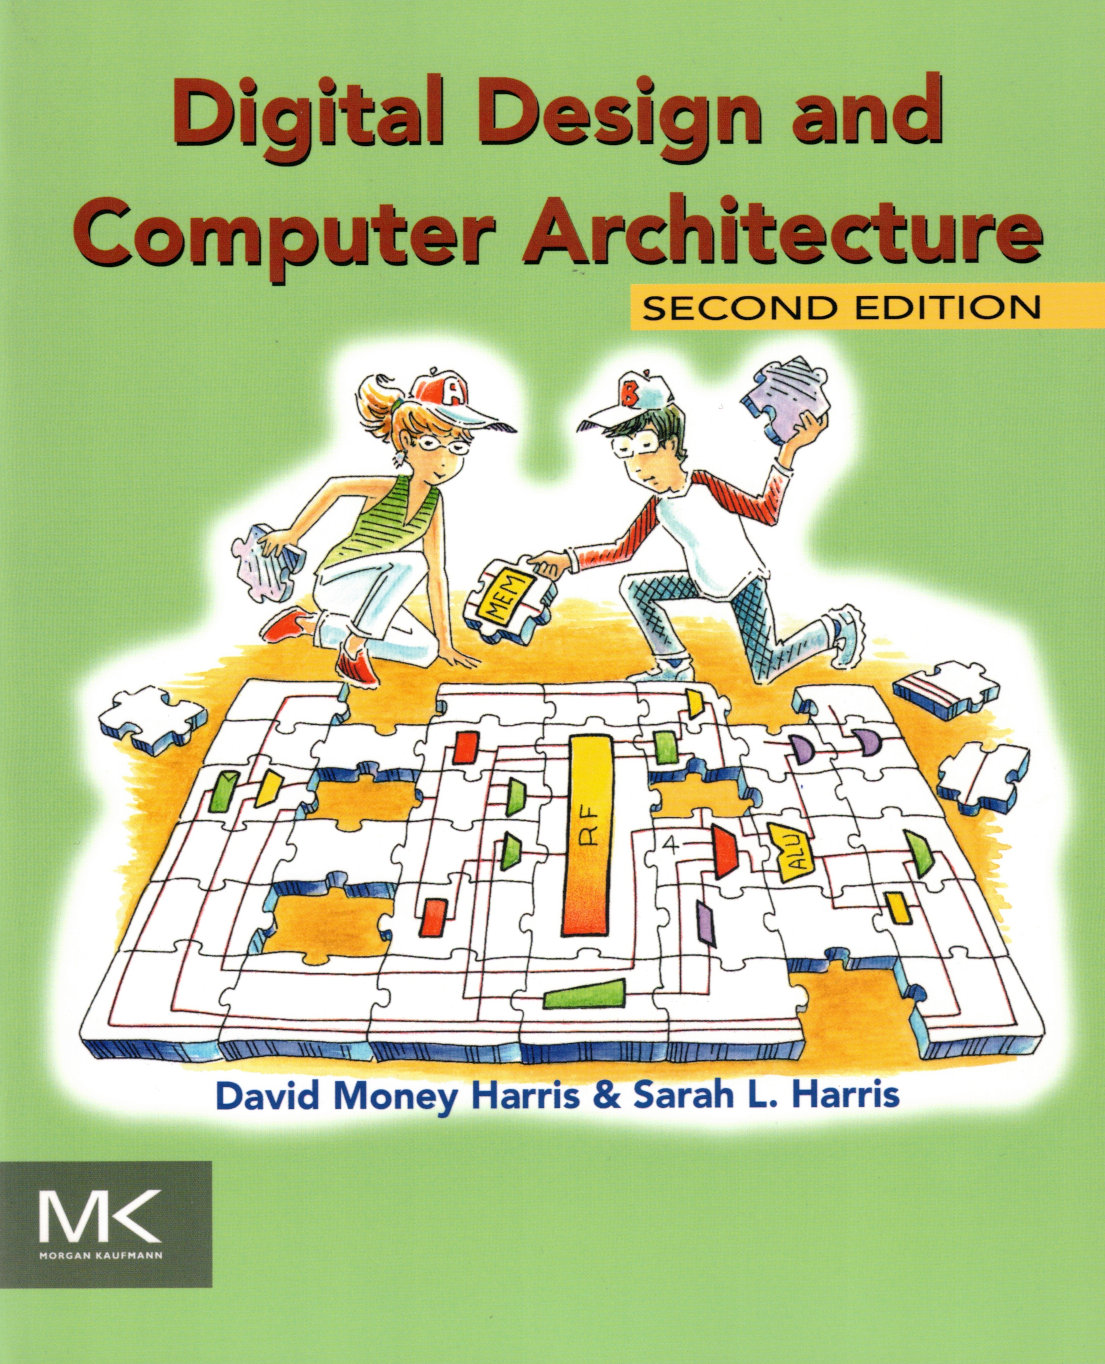
\includegraphics[height=.9\textheight]{gfx/cover_harris_harris.jpg}
    \end{center}
\end{frame}

\begin{frame}

  \frametitle{Your First Real CPU}

  \cpause
  \begin{itemize}
    \item Don't design your own architecture from scratch \cpause
    \item Don't try to build an x86 or ARM \cpause
    \item We want an architecture with
      \begin{itemize}
        \item small footprint of base instructions
        \item well documented
        \item well supported by tooling (especially compilers)
      \end{itemize}
  \end{itemize}
\end{frame}

\begin{frame}
  \frametitle{RISC-V}

  
\includegraphics[height=2em]{gfx/riscv-logo.jpg}
  \vspace{2em}
  \cpause

  \begin{itemize}
    \item Free and Open Source Architecture
    \item Development started in 2010s at Berkeley University
    \item Rich software ecosystem
    \item Actual hardware implementations are becoming available
    \item Especially popular in China
  \end{itemize}
\end{frame}

\begin{frame}
  \frametitle{Why RISC-V?}

  \begin{itemize}
    \item Modular design with optional extensions \cpause
    \item Base instruction set of 40 instructions (RV32I) \cpause
    \item Many useful extensions are small (RV64I, M, Zicsr) \cpause
    \item Allows you to arrive at a working CPU quickly and then focus on specific areas that interest you most (floating-point, vectorization, atomics, \dots) \cpause
    \item Real-world software is deployable also on very limited designs
  \end{itemize}
\end{frame}

\begin{frame}
  \frametitle{Getting Started with RISC-V}

  \href{https://docs.riscv.org/reference/isa/_attachments/riscv-unprivileged.pdf}{Reference Manual}

  \vspace{2em}
  \cpause

  \begin{itemize}
    \item Start with decoding; R32VI was designed with decoding in mind
    \item \href{https://luplab.gitlab.io/rvcodecjs/}{Online Decoder} \cpause
    \item Reference manual already groups instructions by different hardware units, so you can usually implement a chapter on its own \cpause
    \item Instructions are simple enough that you can eyeball test them manually. Regressions are unlikely as you rarely need to touch a component once it is finished.

  \end{itemize}
\end{frame}

\begin{frame}

  \frametitle{Deploying To Your CPU}

  \begin{itemize}
    \item \texttt{clang -O0 --target=riscv32-unknown-none-elf -march=rv32i -mabi=ilp32 -ffreestanding -nostdlib -c main.c -o main.o}
    \cpause \vspace{.5em}
    \item \texttt{ld.lld -T linker\_script.ld main.o -o main.elf}
    \cpause \vspace{.5em}
    \item \texttt{llvm-objcopy -O binary main.elf main.bin} \cpause \vspace{1em}
  \end{itemize}

  Remember that \texttt{-S} gives you the assembly file for debugging

  \href{https://docs.riscv.org/reference/abi/v1.0/riscv-cc-register-convention.html}{Register names in assembly follow a different naming convention}

\end{frame}

\begin{frame}

  \frametitle{Bootstrapping}

  You are running on bare metal.

  \begin{itemize}
    \item Clang code assumes that the hardware is initialized correctly (in particular stack pointer)
    \item Code may reside at the wrong address and needs to be copied by the loader before execution
    \item Bootstrapping entry point needs to be written in assembly, but can jump to high-level code rather quickly
  \end{itemize}


\end{frame}

\begin{frame}

  \frametitle{Compiler Runtime and Standard Library}

  Clang may generate code that relies on symbols that are not defined:
  \begin{itemize}
    \item Arithmetic, such as \texttt{\_\_mulsi3}, \texttt{\_\_divsi3} in case of missing M extensions
    \item Standard library functions such as \texttt{memcpy}, \texttt{memset}, \texttt{memcmp}
  \end{itemize}

  Implement them in software as needed

  \vspace{1em}

\end{frame}

\begin{frame}

  \frametitle{Validation}

  Bare metal debugging works fine in the beginning, but is tedious if a complex C program starts misbehaving.
  \vspace{1em}
  \begin{itemize}
    \item Complete test suite of architecture tests available at \href{https://github.com/riscv/riscv-arch-test}{ https://github.com/riscv/riscv-arch-test.git}
    \item Legacy compliance tests available at \href{https://github.com/lowRISC/riscv-compliance}{https://github.com/lowRISC/riscv-compliance}
    \item Legacy tests are probably enough to iron out most bugs on a simple RV32I
  \end{itemize}
\end{frame}

\begin{frame}
  \frametitle{Lessons to be learned}

  In hardware design, parallelism is key to efficiency.
  \vspace{2em}
  \begin{itemize}
    \item Breaking down complex tasks into simple components similar to software
    \item Reducing delay in a circuit becomes difficult pretty fast
    \item Parallelism is free in HW and does not come with the same issues as in SW
    \item Thinking about optimizing hardware helps build intuition for parallelism
    \item Helps to understand design decisions made by hardware designers better
  \end{itemize}
\end{frame}

\begin{frame}

  \frametitle{Moving on from there\dots}

  Software:
  \begin{itemize}
    \item Support libraries for interacting with peripherals
    \item Porting existing software to your custom machine
    \item Operating System functionality, moving away from bare metal (RISC-V privileged)
  \end{itemize}
  \vspace{1em} \cpause
  Hardware:
  \begin{itemize}
    \item Floating point, Vectorization
    \item Out-of-order execution, pipelining
    \item Concurrency, atomics
    \item High-bandwidth accelerators, GPUs
    \item Serious hardware desing, VHDL, Verilog
  \end{itemize}
\end{frame}

\begin{frame}
  \frametitle{Thanks for your attention.}

  \href{https://stackoverflow.com/users/577603/comicsansms}{
\includegraphics[height=.05\textheight]{../resources/so-icon.png}}
  \href{https://github.com/ComicSansMS}{
\includegraphics[height=.05\textheight]{../resources/github-icon.png}}
  \href{https://bsky.app/profile/comicsansms.bsky.social}{
\includegraphics[height=.05\textheight]{../resources/Bluesky_Logo.png}} ComicSansMS /
  \href{mailto:cpp@andreas-weis.net}{\raisebox{-0.25em}{
\includegraphics[height=.06\textheight]{../resources/email-icon.png}} cpp@andreas-weis.net}

\end{frame}


\end{document}
